%version of 05-05-20

\chapter{Solution Sketches for $\oplus \oplus$ Exercises}
\label{ch:Exercises}


%\section*{Exercises: Chapter 2}

\begin{itemize}
\item
{\bf 2.2. Meeting people at a party}

\smallskip

{\bf To prove}. {\em Some two attendees shake the same number of hands.}

\medskip

The pigeonhole principle is our main tool here.  To wit, the number of people that each attendee {\em does not know} belongs to the set $\{ 0, 1, \ldots, 2n-2 \}$, because each person knows him/herself and his/her partner.  

\smallskip

Because there are $2n$ handshakers (the pigeons) and $2n-1$ hands to shake (the boxes), some two shakers must shake the same numbers of hands.  \qed
 
\medskip
\item
{\bf 2.4. Bi-colored necklaces in tubes}

\smallskip

A {\it bicolored necklace} is composed of $2n = 2(a+b)$ jewels: $2a$ black jewels and $2b$ white jewels.  Let us be given such a necklace within a solid tube of the sort depicted in Fig.~\ref{fig:sample-necklace}, which contains precisely half of the jewels, i.e., $n$ jewels.

\ignore{************************
 For illustration, the necklace in Fig.~\ref{fig:sample-necklace} has $n = 6$, $a = 5$, and $b =1$.
\begin{figure}[ht]
\begin{center}
       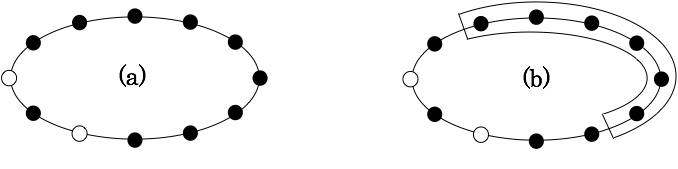
\includegraphics[scale=0.35]{FiguresMaths/SampleNecklace}
\caption{(a) A necklace having $12$ jewels: $10$ black and $2$ white.  (b) The necklace in a tube.}
\end{center}
\end{figure}

In part (a) of the figure, the necklace is unadorned; in part (b), the necklace appears within a length-$n$ {\it tube} which isolates one string---i.e., half-necklace---of $n$ jewels from the complementary string.
*******************************}
\smallskip

{\bf To prove}.
{\em There is a way to position the tube so that both inside the tube and outside the tube, there are: equally many jewels, equally many black jewels, and equally many white jewels.} 

\medskip

We are going to slide the tube clockwise around the necklace, one jewel per step, and count the black jewels and the white jewels within the tube at each step.  Of course, if there are currently equally many black jewels inside the tube and outside the tube, then, by simple arithmetic, we are done---we have the desired ideal position of the tube.  Otherwise, the tube currently has either too many black jewels or too few.  Say, with no loss of generality, that there are too many 
black jewels inside the tube, namely, $a+c$ black jewels for some $c>0$; there is, therefore, a
complementary number of white jewels, namely, $b-c$.  At the end of the process, the tube must contain $a$ black jewels and $b$ white jewels---so the discrepancy $c$ must have been reduced to $0$.  To see that this will eventually happen, we must see how the discrepancy $c$ changes in a single step of the process.

\smallskip

The effect of a single shift is to insert a jewel into the tube, at its advancing extremity, and to eliminate a jewel from the tube, at its trailing extremity.  The discrepancy can be changed by this shift in precisely three ways.
  \begin{itemize}
  \item
If the inserted jewel and the eliminated jewel are of the same color, then the discrepancy $c$ 
is unchanged by this shift.
  \medskip\item
If the inserted jewel is black and the eliminated jewel is white, then the discrepancy $c$ is {\em increased to} $c+1$ by this shift. 
  \medskip\item
If the inserted jewel is white and the eliminated jewel is black, then the discrepancy $c$ is {\em decreased to} $c-1$ by this shift. 
  \end{itemize}
By the time $n$ shifts have been performed, the discrepancy $c$ will have changed to $-c$, because the tube will be in an antipodal position upon the necklace.

\smallskip

Summing up: Over the course of $n$ shifts, the discrepancy $c$ will have changed to $-c$.  The  discrepancy changes by $\pm 1$ at each shift.  Therefore, there must be some shift among the $n$ when the discrepancy is $0$.  \qed
 

\medskip \item
{\bf 2.6. Using {\em geometric} intuition to sum inverse powers of $4$}

\smallskip

We seek a proof of Proposition~\ref{thm:sumof-1/4-induction} in which the infinite summation
\[ S \ \ = \ \  {1 \over 4} \ + \  {1 \over 4^2} \ + \cdots + \ {1 \over 4^k} \ + \cdots  \]
is analyzed---and ultimately solved---geometrically.  The key is to discover how to represent the process of generating successive inverse powers of $4$.  The nested similar triangles in Fig.~\ref {Fig:Sumgeosimilar} unlock the secret to this representation.
\begin{figure}[ht]
\begin{center}
        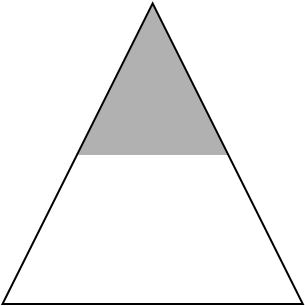
\includegraphics[scale=0.3]{FiguresMaths/Sum1over4topTriangle}
        \hspace{1cm}
        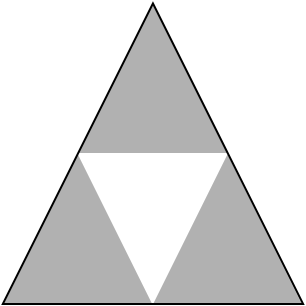
\includegraphics[scale=0.3]{FiguresMaths/Sum1over4similarTriangles}
\caption{Two copies of an isosceles triangle $T$.  The lefthand copy has been partitioned into a top sub-triangle , call it $T'$, whose height is half of $T$'s.  The righthand copy is obtained by adding two copies of $T'$ in the lower half of the lefthand copy.  We now have four similar copies of $T'$ within $T$, which perfectly partition the area of triangle $T$.}
        \label{Fig:Sumgeosimilar}
\end{center}
\end{figure}


\ignore{***************
We prove in Proposition~\ref{thm:sum-finite-geometric-series}(b) that this infinite summation converges to the value ${1 \over 3}$.  
A simple way to see this is to multiply the summation $S$ term by term by the fraction $1/4$.  We observe---just by inspection---that the resulting product, which clearly has the value $S/4$, equals $S - 1/4$, so that $S = 1/3$.
\smallskip
*************************}
\begin{itemize}
\item
{\bf To prove}. {\em The four sub-triangles are similar to one another.}

\smallskip

Duplicate triangle $T'$ twice, and put both copies at the bottom of triangle $T$, in the manner depicted in Fig.~\ref{Fig:Sumgeosimilar}(right).  The reversed, white, sub-triangle in the middle of the figure has the same sides as the two duplicates of $T'$, and its base is also half of $T$'s.  Therefore, it also is similar to triangle $T'$.

\medskip\item
{\bf To prove}. {\em The four sub-triangles are similar to triangle $T$.}

\smallskip

Sub-triangle $T'$ is similar to triangle $T$ because it is obtained by bisecting both the base and the sides of $T$.

\medskip\item
{\bf To prove}.  {\em The common area of each of the four sub-triangles is $1/4$ the area of $T$.}

\smallskip

This follows from the two previous observations: The four sub-triangles have the same area,
and they exactly cover triangle $T$. 
\end{itemize}

\medskip\item
{\bf To do}. {\em Assemble the preceding facts into an evaluation of the sum $S$.}

\smallskip

The sum $S$ is obtained by recursively partitioning the small upper sub-triangles. 

The process splits the original triangle into layers that each contain three sub-triangles; see
Fig.~\ref{Fig:Sum1over4FirstLayer}). 
\begin{figure}
\begin{center}
        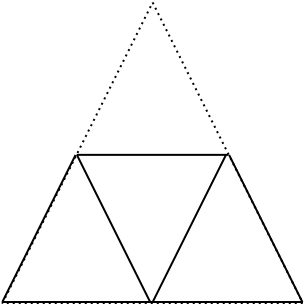
\includegraphics[scale=0.3]{FiguresMaths/Sum1over4FirstLayer}
        \caption{First bottom layer of the partitioning..}
        \label{Fig:Sum1over4FirstLayer}
\end{center}
\end{figure}
As the three sub-triangles are identical, the area of the central reversed triangle is $1/3$ of the area of the layer. 

\smallskip

The final solution is depicted in Fig.~\ref{Fig:Sum1over4cascade}, where the recursive process is applied ``all the way". 
\begin{figure}
\begin{center}
        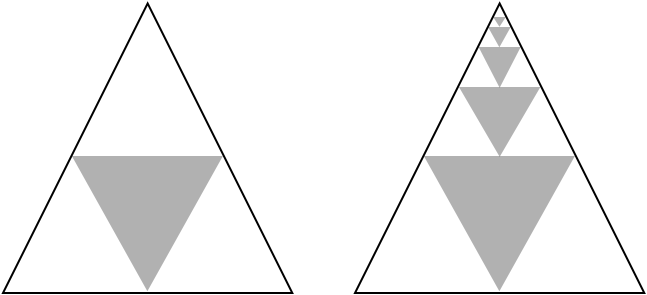
\includegraphics[scale=0.3]{FiguresMaths/Sum1over4cascade}
        \caption{The recursive decomposition of triangle $T$.}
        \label{Fig:Sum1over4cascade}
\end{center}
\end{figure}
Summarizing  the graphical construction.  If the area of the original triangle $T$ is $1$, then 
the area of the grey sub-triangle of Fig.~\ref{Fig:Sum1over4cascade}(left) is $1/4$, since it is one of four identical triangles.  Then, because each grey triangle in Fig.~\ref{Fig:Sum1over4cascade}(right) occupies one-third of the area of its layer of, the aggregate area of the grey sub-triangles is $1/3$ of the area of $T$.  One can now apply Fubini's principle to evaluate the sum $\sum_{k \geq 1} \ 4^{-k}$.
\end{itemize}

\ignore{*************************
\subsection{A graphical proof}

\noindent \textit{The problem.}
%\label{thm:an-arithmetic-identity}
Prove the following property:

or any positive integer $n$,
\[ \Delta_{2n-1} \ = \ n + 4 \Delta_{n-1}. \]
\medskip

\noindent \textit{The solution.}

Consider the arithmetic series in (\ref{eq:arith-seq}) for the case
$a=1$ and $b=4$.  
By Proposition~\ref{thm:sum-of-arithmetic-series},
this series, call it $S^{(1,4)}(n)$, has the sum
\begin{equation}
\label{eq:triangles}
S^{(1,4)}(n) \ = \ n + 4 \Delta_{n-1}.
\end{equation}

Let us represent the sum $\Delta_{n-1}$ in the natural way as a
triangle of tokens.  This triangle has a base of $n-1$ tokens, upon
which sits a row of $n-2$ tokens, upon which sits a row of $n-3$
tokens, \ldots, all the way to the apex, which has a single token.

Now, let us view equation (\ref{eq:triangles}) as giving us access to four
copies of the preceding triangle of tokens.  Let us arrange these
triangles in the manner depicted in Fig.~\ref{fig:Delta(n)4}.
\begin{figure}[ht]
\begin{center}
       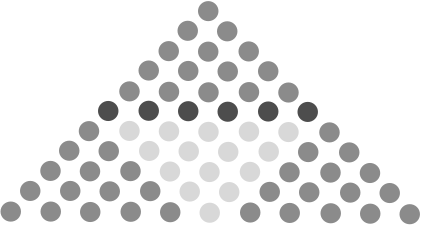
\includegraphics[scale=0.5]{FiguresMaths/Delta4}
 \caption{Arranging the four triangles plus a row to obtain a new (bigger) triangle.}
       \label{fig:Delta(n)4}
\end{center}
\end{figure}
Now, ``complete the picture'' by adding an ``extra'' row of $n$
tokens at row $n$ of the figure (these are depicted in dark gray in
the figure).  The four small triangles, augmented by the ``extra'' row
of $n$ tokens has clearly become a representation  of $\Delta_{2n-1}$
by tokens.

We now have a purely pictorial proof of the proposition. 

*************************}


%%%%%%%%%%%%%%%%%%%%%%%%%%%%%%%%%%%%%%%%%%%%%%


%\section*{Exercises of Chapter 3}

\begin{itemize}
\item
{\bf 3.8. More connections between strings and functions}
\medskip

{\bf To do}.  {\em Craft an argument that predicts the number of permutations, based on the size of set $S$.}
\smallskip

  \begin{itemize}
  \item
As you create a new string of numbers, in how many ways can you choose {\em the first number}? {\em the second number}? \ldots

\smallskip

There are $n$ ways to choose the first element of the permutation.  Independently of which first element has been chosen, there remain $n-1$ ways to choose the second element. Independently of which elements are chosen as the first two, there remain $n-2$ ways to choose the third element.  And so on \ldots

  \medskip\item
Based on your answers for the first and second and third numbers of the new string, in how many ways can you choose {\em the first two numbers---i.e., the first {\em pair} of numbers}?  {\em the next pair of numbers}? \ldots

\smallskip

The main message here is that {\em independent} choices {\em multiply}.  This means that the $n$ choices for element \#1 and the $n-1$ choices for element \#2 lead to
\[ n(n-1) \]
ways to choose the first pair of numbers.  The persistence of independence of successive selections means that the multiplicative rule continues to hold: There are $n(n-1)(n-2)$ ways to choose the first triple of elements,
\[ n(n-1)(n-2)(n-3) \]
ways to choose the first quadruple of elements, \ldots
  \end{itemize}

{\bf To do}. {\em Strengthen your argument by listing all permutations of  $S' =  \{1,2,3,4,5\}$.}

\smallskip

The challenge is to convert your mathematical reasoning into a systematic method of
enumeration.  Here is a natural recursive way of doing this. (i) Fix the first number (among the 5 possibilities).  (ii) Recursively, enumerate, for each copy of the first number, all permutations of the four remaining numbers.

\smallskip

{\bf To do}. {\em Extrapolate from your argument to determine the number of permutations of the set $S" =  \{1,2,3, \ldots, n\}$, as a function of $n$.}

\smallskip

$Fact(n) \ = \ n \times Fact(n-1) \ = \ n \times (n-1) \times \cdots \times 2 \times 1$.

\end{itemize}


%%%%%%%%%%%%%%%%%%%%%%%%%%%%%%%%%%%%%%%%%%%%%%%%
%\section*{Exercises: Chapter 4}

\begin{itemize}
\item
{\bf 4.5. The rationals ($\Q$) and the integers ($\N$) are equinumerous}
\smallskip

{\bf To prove}. {\em Provide a {\em detailed} proof of Proposition~\ref{thm:|Q|=|N|}:} 
There are ``equally many" integers as there are rationals.

\smallskip

The relevant fact here is that $\Q$ is (isomorphic to) a proper subset of $\N \times \N$.  One bijection that witnesses this fact is defined as follows.  Map each rational $r \in \Q$ to the unique pair $\langle p,q \rangle \in \N \times \N$ such that:
\[ [r = p/q] \ \ \  \mbox{ and } \ \ \  [\mbox{$p$ and $q$ share no common factor}] \]

\smallskip

Beware: The first of these conditions is satisfied by infinitely many pairs of integers.  The second condition is needed to end up with a unique pair, hence with the desired bijection.

\smallskip

Once you have a bijection, you can argue based on definitions.
\end{itemize}


\ignore{***************************************
\subsection{Complex
  multiplication via $3$ real multiplications}
\index{complex number!multiplication via 3 real multiplications}

\noindent {\it The problem.}
%\label{thm:complex-mult-3real}
Show how to compute the product of two complex numbers using only {\em three}
real multiplications rather than four.
\medskip

\noindent {\it The solution.}
Although implementing (\ref{eq:complex-mult}) ``directly'' correctly
produces the product $\kappa = (a+bi) \cdot (c+di)$, there is another
implementation that is {\em more efficient}.  Specifically, the
following recipe computes $\kappa$ using only {\em three} real
multiplications instead of the four real multiplications of the
``direct'' implementation.  We begin to search for this recipe by
noting that our immediate goal is to compute both Re$(\kappa) = ac-bd$
and Im$(\kappa) = ad+bc$.  We can accomplish this by computing the
{\em three} real products
\begin{equation}
\label{eq:complex-mult-3a}
(a+b) \cdot (c+d); \ \ \ \ \
ac;  \ \ \ \ \ bd
\end{equation}
and then noting that
\begin{equation}
\label{eq:complex-mult-3b}
\begin{array}{lcl}
\mbox{Im}(\kappa) & = & (a+b) \cdot (c+d) - ac -bd, \\
\mbox{Re}(\kappa) & = & ac -bd
\end{array}
\end{equation}
We thereby achieve the result of the complex multiplication described
in (\ref{eq:complex-mult}) while using only {\em three} real
multiplications.


%%%
\subsection{Another proof for irrationality of $\sqrt{2}$}


\noindent \textit{The problem.}
Prove the irrationality of $\sqrt{2}$ using a geometrical argument.
\medskip

\noindent \textit{Hint.}
The proof is by contradiction. 

Consider $\sqrt{2}$ is rational, which means there exists a pair of integers $(a,b)$
such that $\sqrt{2} = \frac{a}{b}$ (where $a$ is larger than $b$).
Among all possible pairs, take the unique irreductible ratio.

Represent this expression geometrically by the corresponding isosceles triangle
which is the one of minimal surface. 

The contradiction comes by constructing another isosceles triangle with a smaller surface.
%Squaring this expression leads to $2.b^2 = a^2$.
\medskip

\noindent \textit{The solution.}

The solution is depicted in Fig.~\ref{Fig:sqrtbisInit} and~\ref{Fig:sqrtbisFin} . 
\begin{figure}
\begin{center}
        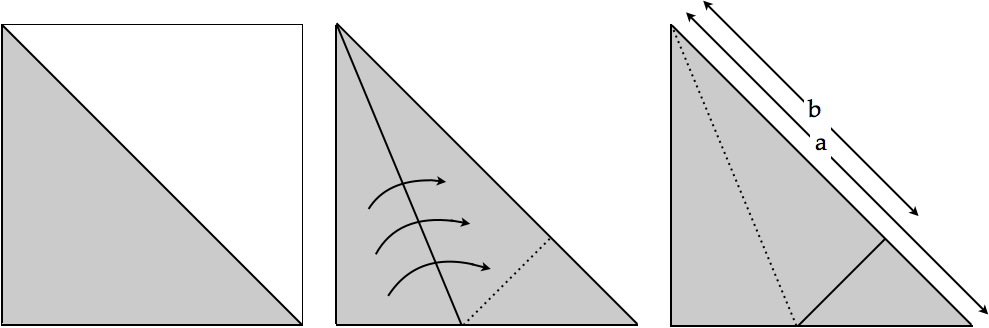
\includegraphics[scale=0.3]{FiguresArithmetic/sqrtbisInit}
        \caption{First step: folding the triangle along the side.}
        \label{Fig:sqrtbisInit}
\end{center}
\end{figure}
\begin{figure}
\begin{center}
        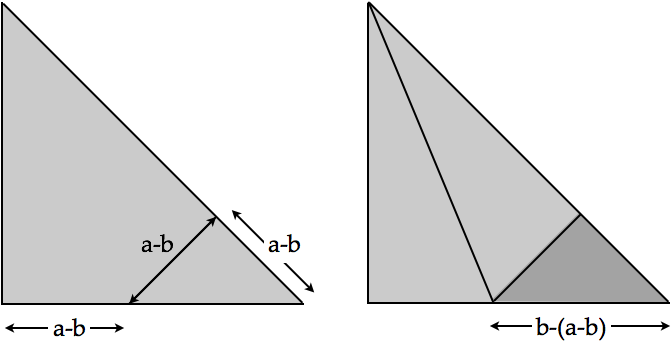
\includegraphics[scale=0.3]{FiguresArithmetic/sqrtbisFin}
        \caption{Second step. The sides of the small isosceles triangle are integers.}
        \label{Fig:sqrtbisFin}
\end{center}
\end{figure}
****************************}


%%%%%%%%%%%%%%%%%%%%%%%%%%%%%%%%

\ignore{*******************************
\section{Chapter 5}


\subsection{A ``trick'' for squaring certain integers}


\noindent \textit{The problem:}

Let $n$ be any number that has a $2$-digit decimal numeral of the form

\hspace{.25in}$5.\delta$ \ \ \ \ $(\delta \in \{ 0,1,2,3,4,5,6,7,8,9\})$.

\noindent
Then the square of $n$ is the integer

\hspace{.25in}$25 \ + \ \delta \cdot (\delta +1)$
\medskip

\noindent \textit{The solution:}

We can rewrite the premise of the proposition in the form
\[ n \ = \ 10 \cdot \delta + 5 \]
It is now easy to invoke Proposition~\ref{prop:(a+b)(c+d)} and the
distributive law to compute that

\[ n^2 \ = \ 100 \cdot \delta \cdot (\delta+1) + 25 \]
To wit: 
\[
\begin{array}{lclll}
n^2 & = & (10 \cdot \delta + 5)^2 & & \mbox{Given} \\
    & = & 100 \cdot \delta^2 \ + \ 100 \cdot \delta \ + \ 25
              & & \mbox{the proposition} \\
    & = & 100 \cdot (\delta^2 \ + \ \delta) \ + \ 25
              & & \mbox{factoring: distributive law} \\
    & = & 100 \cdot \delta \cdot (\delta + 1) \ + \ 25
              & & \mbox{factoring: distributive law} \\
\end{array}
\]
A parlor trick has become a mathematical demonstration!


%%%
\subsection{Revisiting a very old problem}

\noindent \textit{The problem:}

This problem comes from babylonians in the 18th century BC.
The numeral system was in base 60, and the problem was to determine the length of the side of a square which was part of a larger rectangle.
The following figure details the process.
\medskip

\noindent \textit{The solution:}

The idea of the proof is to represent the left hand side by the square $x^2$ beside a rectangle $60 \times x$
(see Fig.~\ref{fig:equationBabillon}).
Recall that the coefficient of $x$ in the equation is $1$, this corresponds to $60$ in the considered basis. 
Then, split the right rectangle into two equal parts and move one part a the bottom of the left square.
The final figure shows the whole square whose surface is equal to $45$ plus the surface of the white square
whose surface is equal to $30 \times 30$.
In base $60$, this is equal to $15$. 
$45+15 = 60$, thus, the big square is the unit square, its side is $60$.
Thus, the length of the initial square is equal to $60-30=30$.
\begin{figure}[htb]
\begin{center}
       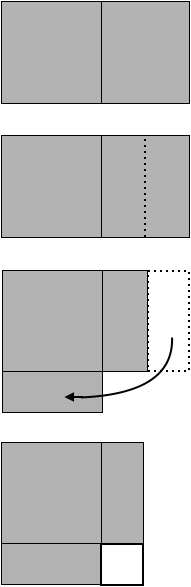
\includegraphics[scale=0.4]{FiguresArithmetic/tabletteMesopotamie}
\caption{Solving $x^2 + x = 45$.}
\label{fig:equationBabillon}
\end{center}
\end{figure}
*****************************}


%%%%%%%%%%%%%%%%%%%%%%%%%%%%%%%%%%%%%%%%%%

%\section*{Exercises: Chapter 6}

\begin{itemize}
\item
{\bf 6.4. How to evaluate $S_1(n) = \sum_{i=1}^n \ i$, using a ``machine" which evaluates $S_2(n) = \sum_{i=1}^n \ i^2$}
\smallskip

{\bf To do}. {\em Show how to use the $S_2(n)$-machine in order to compute $S_1(n)$.}

\medskip

You must exploit how the expressions for $S_1(n)$ and $S_2(n)$ relate to one another.  (You need just a little algebra here.)  Then you must exhibit how to extract the relation from a ``machine" which gives out values in a ``black-box" manner.

\smallskip

You can develop the solution strategy as follows:  
Write the summation $S_2(n+1)$ in two ways.  First, isolate the {\em last} term of the summation; then, isolate the {\em first} term of the summation:
\begin{eqnarray*}
S_2(n+1) & = &  \sum_{i=1}^{n} i^2 \ + \ (n+1)^2  \\
                & = & S_2(n) \ + \ (n+1)^2 \\
S_2(n+1) & = & 1 \ + \sum_{i=2}^{n+1} i^2 \\
                & = & 1 \ + \sum_{i=1}^{n} \ (i+1)^2 \\
                & = & 1 \ + \sum_{i=1}^{n} \ (i^2 \ + \ 2 i \ + \ 1) \\
                & = & 1 \ + \ S_2(n) \ + \ 2 S_1(n) \ + n
\end{eqnarray*} 
Equating the two final derived expressions for $S_2(n+1)$ and simplifying, we find that
\begin{eqnarray*}
 S_2(n) \ + \ (n+1)^2 & = & 1 \ + \ S_2(n) \ + \ 2 S_1(n) \ + n \\
                    (n+1)^2 & = & 1 \ + \ 2 S_1(n) \ + n \\
                  2 S_1(n) & = & (n+1)^2 \ - \ (n + 1) \\
                     S_1(n) & =  & \frac{1}{2} \ n(n+1) 
\end{eqnarray*} 

\medskip
\item
{\bf 6.6. Evaluating a geometric summation pictorially}

\smallskip

\ignore{***************
In Section~\ref{sec:summing-geometric-series:techniques}, we used Thales's theorem about similarity in triangles (Theorem~\ref{thm:Thm-of-Thales-similarity}) to sum the simple infinite geometric series $\sum_{i=0}^\infty \ b^i$.  It turns out that a modest modification of that evaluation strategy allows us also to evaluate the truncated versions of that series, namely, the summations
\[ S^{(b)}(n) \ = \ \sum_{i=0}^n \ b^i \]
************************}

{\bf To do}. {\em Use the following figure to evaluate the following summation.}
\[ S^{(b)}(n) \ = \ \sum_{i=0}^n \ b^i \]

\centerline{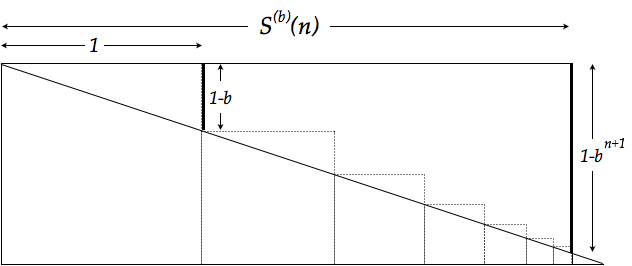
\includegraphics[scale=0.4]{FiguresArithmetic/ThalesGeometricSumFiniteSol}}
\smallskip

We use Thales's Theorem~\ref{thm:Thm-of-Thales-similarity} with the two upper similar triangles in the figure.
\[ \frac{S^{(b)}(n)}{1-b^{n+1}} \ = \ \frac{1}{1-b} \]
\[ S^{(b)}(n) \ = \ \frac{1-b^{n+1}}{1-b} \]

\medskip
\item
{\bf 6.7. A direct proof that the harmonic series diverges}

{\bf To do}.  {\em Develop a proof of the divergence of the harmonic series }

\[ S^{(H)} \ = \ \sum_{k=1}^\infty \ {1 \over k} \]

\begin{enumerate}
\item
Partition $S^{(H)}$'s terms into groups whose sizes are successive powers of $2$
\item
Develop an argument based on the sums within the groups.
\end{enumerate}

\smallskip

The partitioning step operates as follows:
{\footnotesize
\[ 
\begin{array}{ll}
S^{(H)}   & = \ 1  + {1 \over 2} + \left(  {1 \over 3}   +  {1 \over 4}  \right) + \left( {1 \over 5} + {1 \over 6}+ {1 \over 7}  +  {1 \over 8} \right) + \left( {1 \over 9} + {1 \over 10}+ {1 \over 11}  +{1 \over 12} + {1 \over 13} + {1 \over 14} + {1 \over 15} + {1 \over 16} \right) \ +\cdots
\end{array} \]
}

In detail, each group, say the $i$th group $G_i$ (for $i \geq 1$), is computed from the $i$ numbers
\[ \frac{1}{2^{(i-1)}+1}, \ \frac{1}{2^{(i-1)}+2}, \ \ldots, \ \frac{1}{2^{i}}  \]
Grouping the terms in the earlier manner, the sum within each group $G_i$ exceeds $1/2$:
\begin{eqnarray*}
{1 \over 3} + {1 \over 4} \ > \ 2 \cdot {1 \over 4} & = & {1 \over 2} \\ \smallskip
{1 \over 5} + {1 \over 6} + {1 \over 7}+ {1 \over 8} \ > \ 4 \cdot {1 \over 8} & = & {1 \over 2}  \\  \smallskip
{1 \over 9} + {1 \over 10} + {1 \over 11}  +{1 \over 12} + {1 \over 13} + {1 \over 14} + {1 \over 15} + {1 \over 16}  \ > \ 8 \cdot {1 \over 16} & = & {1 \over 2}  \\  \smallskip
\vdots
\end{eqnarray*}
Therefore, 
\begin{eqnarray*}
S^{(H)} & > & 1 \ + \ \left( {1 \over 2} \ + \ {1 \over 2} \right) \ + \left( {1 \over 2} + {1 \over 2} \right) + \cdots \\
             & = & 1 \ + \ 1 \ +  1 \ + \ 1 \ + \cdots
\end{eqnarray*}
This means that the Harmonic sum $S^{(H)}$ is greater than every sum of $1$s, hence, is infinite.

\medskip

{\bf To do}. {\em Propose an alternative analysis of $S^{(H)}$ which uses groupings whose sizes are multiples of $3$}

\smallskip

The aim of this problem is to ensure that you have understood which features of our power-of-$2$ groupings are inherent to the argument and which are just for convenience.

\smallskip

We argue now in a somewhat different way than with our power-of-$2$ groupings.  We now propose the terms $S_i$ defined by
\[ 
S_i \ = \ \left( \frac{1}{3i-1} + \frac{1}{3i} + \frac{1}{3i+1} \right) \ >  \ 3 \cdot \frac{1}{i}
 \]
We then have
\begin{eqnarray}
\nonumber
S^{(H)}  & = & 1 + S_1 +  S_2 + \cdots + S_i + \cdots  \\
\label{eq:harmonic-by-3}
             & >  & 1 + 3 \cdot \frac{1}{3} + 3 \cdot \frac{1}{6} + \cdots + 3 \cdot \frac{1}{3i} + \cdots
\end{eqnarray}

These summations lead to the following absurdity.

\smallskip

If $S^{(H)}$ were finite, then, by Eq.~\ref{eq:harmonic-by-3}, we would have $S^{(H)}  > 1 + S^{(H)} $, which is obviously impossible. 


\medskip
\item
{\bf 6.8. Summations, and summations of summations}
\smallskip

  \begin{itemize}
  \item a.
{\bf To prove}: 
\[ \widehat{\Theta}_n \ \eqdef \  \sum_{k=1}^n \ \Delta_k \ = \   
\Delta_1 + \Delta_2 + \cdots + \Delta_n \ = \ \frac{1}{3} \Delta_n \cdot (n+2) \]

The result is obtained by replacing each triangular number $\Delta_k$ in the summation by its explicit expression, and then perform the indicated algebraic manipulation.  We thereby find:
\begin{eqnarray*}
\widehat{\Theta}_n & = & \sum_{k=1}^n \ \frac{k(k+1)}{2} \\
    & = & \frac{1}{2} \sum_{k=1}^n k^2  + \frac{1}{2} \sum_{k=1}^n k  \\
    & = & \frac{1}{2} \ \left( \frac{n (2n+1) (n+1)}{6} \ + \ \frac{n (n+1)}{2} \right)\\
    & = & \frac{1}{2} \frac{n (n+1)}{2} \cdot \left( \frac{2n+1}{3} + 1 \right)  \\
    & = & \frac{1}{2} \Delta_n \cdot \frac{(2n+4)}{3}  \\
    & = & \Delta_n \cdot \frac{(n+2)}{3}
\end{eqnarray*} 

%  \item
%{\em Develop and verify a formula for the summation:}
%\[ \Upsilon_n  \ \eqdef \  \sum_{k=1}^n \ \widehat{T}_k \ = \  
%\widehat{T}_1 + \widehat{T}_2 + \cdots + \widehat{T}_n \]

  \item b.
{\bf To prove}.  {\em Verify the following identities involving $\Delta_n$.}

\smallskip

    \begin{itemize}
    \item i.
For all $n \in \N^+$:
$\Delta_n \ + \ \Delta_{n-1} \ = \ n^2$

\smallskip

You can do the necessary algebraic manipulation, but you can alternatively use a pictorial proof, which is a slight modification of our pictorial evaluation of $\Delta_n$. 
\begin{figure}[htb]
\begin{center}
       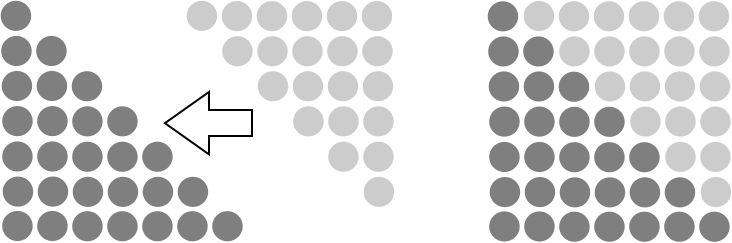
\includegraphics[scale=0.3]{FiguresMaths/DeltaSumSquare}
\caption{Summing $\Delta_n$ and $\Delta_{n-1}$ to obtain the $n \times n$ square.}
%\label{fig:}
\end{center}
\end{figure}

   \item ii.
For all $n \in \N^+$:
$\Delta_n^2 \ - \ \Delta_{n-1}^2 \ = \ n^3$

\smallskip

Write $\Delta_n$ as  $n \ + \ \Delta_{n-1}$:
\begin{eqnarray*}
\Delta_n^2 \ - \ \Delta_{n-1}^2 & = & \left( n \ + \ \Delta_{n-1} \right)^2 - \ \Delta_{n-1}^2  \\
    & = & n^2 \ + \ 2n \cdot \Delta_{n-1} \ + \ \Delta_{n-1}^2 - \ \Delta_{n-1}^2 \\
    & = & n^2 \ + \ 2n \cdot \frac{n(n-1)}{2}\\
    & = & n^2 + n^3 - n^2 \\
\end{eqnarray*} 
\end{itemize}

  \item c.
{\bf To do}.  {\em Derive a closed-form expression for the sum}
\[ \widehat{\Theta}_n \ + \ \widehat{\Theta} _{n-1} \]

\smallskip

This question is more open-ended than the previous ones since we don't know \textit{what kind of expression} to look for.

\smallskip

When encountering such open-ended problems, you can never go wrong by starting out with the original definitions.

\smallskip

In this case, we express the tetrahedral number $\widehat{\Theta}_n$ as the sum of triangular numbers.
\begin{eqnarray*}
\widehat{\Theta}_n \ + \ \widehat{\Theta} _{n-1} 
  & = & \sum_{k=1}^n \Delta_k \ + \ \sum_{k=1}^{n-1} \Delta_k \\
  & = & \Delta_1 \ + \ \sum_{k=2}^{n} \left( \Delta_k + \Delta_{k-1} \right)
\end{eqnarray*} 
We can now use the expression we derived for the sum of two consecutive $\Delta_k$s:
\[
\widehat{\Theta}_n \ + \ \widehat{\Theta} _{n-1} \ = \ 1 + \sum_{k=2}^{n} k^2 
\ = \ \sum_{k=1}^{n} k^2 
\]
We can finally replace this summation by its closed-form sum.
\[
\sum_{k=1}^{n} \ k^2 \ = \ \frac{n(n+1)(2n+1)}{6}
\]
  \end{itemize}
\end{itemize} 


\ignore{*****************************
%%%
\subsection{Sum of perfect cubes}

\noindent \textit{The problem.}
Show that the sum of $n$ first cubes is equal to a perfect square, and more precisely, $\Delta_n^2$.
\medskip

\noindent \textit{The solution.}
The proof is based on an hold and simple pattern that we learned in elementary school.
\medskip

\index{$n^2$ as sum of first $n$ odd integers!a proof from elementary school}

%
Consider the following reasoning which emerges from the way
multiplication tables are developed in elementary school.  
Let us first illustrate the idea using the case $n=5$.
\begin{equation}
\label{eq:Fubini-table}
\begin{array}{rrrrr}
1  &  2 &  3 &  4 &  5 \\
2  &  4 &  6 &  8 & 10 \\
3  &  6 &  9 & 12 & 15 \\
4  &  8 & 12 & 16 & 20 \\
5  & 10 & 15 & 20 & 25 \\
\end{array}
\end{equation}
Write the integers $1, 2, \ldots, n$ in a row.  Below this row, write
the doubles of these integers.  Below the ``double'' row, write the
triples of the integers.  Below the ``triple'' row, write the
quadruples of the integers, then the quintuples, and so on.  Note that
the resulting table is {\em symmetric:} its rows are identical to its
columns.
\medskip

Using again Fubini's rearrangement stratagem, we now count all the integers in
the table in two different ways.
\begin{enumerate}
\item
We sum the entries of our table by peeling away successively larger
reversed instances of the letter ``$L$'' (as in our earlier
``pictorial'' proof of
Proposition~\ref{thm:squares-odd-integers-Gauss}).  We find that the
integers in each ``$L$'' sum to a perfect cube.
Actually, the diagonal is (by definition) equals to the square.
\[
\begin{array}{rrrrrrrrr|rrc}
1  &    &    &    &    &   &     &    &   & 1   & = 1^3 \\
2  &  4 &  2 &    &    &   &     &    &   & 8   & = 2^3 \\
3  &  6 &  9 &  6 &  3 &   &     &    &   & 27  & = 3^3 \\
4  &  8 & 12 & 16 & 12 &  8 &  4 &    &   & 64  & = 4^3 \\
5  & 10 & 15 & 20 & 25 & 20 & 15 & 10 & 5 & 125 & = 5^3
\end{array}
\]

\item
We sum the successive rows of the $n \times n$ table (\ref{eq:Fubini-table}).  
The first row of the table sums to $\Delta_n$; the second row sums to $2
\Delta_n$; the third row sums to $3 \Delta_n$; \ldots; the last row sums
to $n \Delta_n$.  
Thus, the aggregate sum of the table's rows is 
\[ (1 + 2 + \cdots + n) \cdot \Delta_n \ = \ \left(\Delta_n \right)^2 \]
\end{enumerate}
We conclude that
\[
\sum_{i=1}^n i^3 \ = \  \left(\Delta_n \right)^2
\]
************************************************}


%%%%%%%%%%%%%%%%%%%%%%%%%%%%%%%%%%%%%

%\section*{Exercises: Chapter 7}


\ignore{****************************
\subsection{Handling asymptotic}


\noindent \textit{The problem.}

Prove that $f = O(g)$ and $h = O(k)$ for functions $f,g,h,k$ implies that
$f+h = O(g+k)$


\subsection{What's wrong?}

\noindent \textit{The aim.}
to investigate a proof which leads to surprising results.


\begin{enumerate}
\item
Let consider the infinite sum $A = 1-1+1-1+ \ldots$

show that $A=\frac{1}{2}$ (hint: compute $1-A$)
\item
Let now consider the other infinite sum $B=2-3+4-5+6 \ldots$

show that $B=\frac{1}{4}$ (hint: compute $A+B-1$)
\item 
Compute the sum of the integers $C=1+2+3+4+ \ldots$

show that $C=-\frac{1}{12}$ (hint: compute $C-B=4+8+12+16+ \ldots$)
\end{enumerate}

\medskip

\noindent \textit{The problem.}

What's wrong?

\medskip

\noindent \textit{The solution.}
First, summing up positive number should be positive, 
and second, the sum of the integers should be infinite...

Then, how to analyze the previous result/proof?
******************************************************}




%%%%%%%%%%%%%%%%%%%%%%%%%%%%%%%%%%


%\section*{Exercises: Chapter 8}

\begin{itemize}

\item
{\bf 8.2. Discovering fractal-like structure in Pascal's triangle}

{\Arny Solution needed}

{\bf To prove}.  {\em The fractal-like structure that we describe now really occurs.}

\smallskip

Pascal's triangle modulo a prime $m$ (where each of the triangle's entries is taken modulo $m$) is illustrated in Fig.~\ref{fig:TriangleFractal}.

\begin{figure}[ht]
\begin{center}
	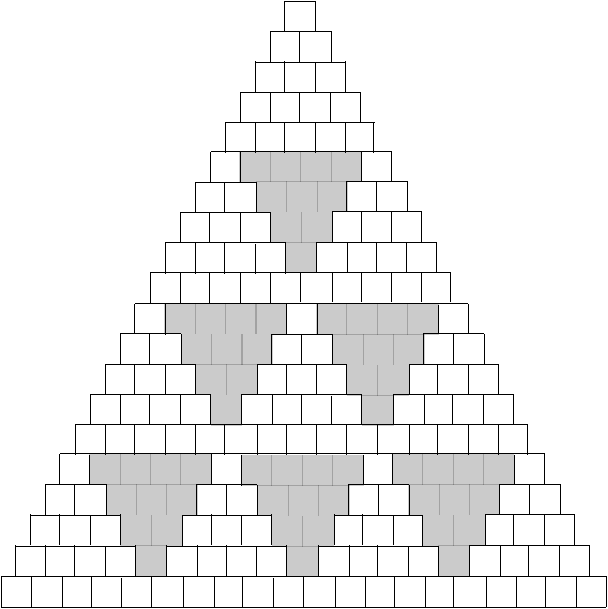
\includegraphics[scale=0.3]{FiguresArithmetic/PascalTriangleFractal.png}
	        \caption{The reproducible patterns in Pascal's triangle modulo $5$.
	        The grey-shaded inverted triangles have entry $0$ in every position.}
        \label{fig:TriangleFractal}
\end{center}
\end{figure}

The first $m$ levels of the triangle replicate endlessly, with periodic inverted $(m-1)$-level triangles whose entries are all $0$.  (In the figure, the inverted triangle of $0$s is depicted in grey.)   One observes that the original triangle becomes a fractal-like repetitive structure whose pattern of repetitions is dictated by the parameter $m$.

%
\medskip\item
{\bf 8.4. Divisibility among integers: via the Fundamental Theorem of Arithmetic}

  \begin{itemize}
\item
b. {\bf The sieve of Eratosthenes and its implications}

We formulate the sieve as a regimen for labeling integers with their prime factors.  For simplicity, we use the label $\lambda_p$ to identify integers which are multiples of prime $p$.

\medskip

The multiples of $2$, $3$ and $5$ are labeled in the following table:

$\begin{array}{c|c|c|c|c|c|c|c|c|c|c|c|c}
1 & 2 & 3 & 4 & 5 & 6 & 7 & 8 & 9 & 10 & 11 & 12 & 13 \\
 & \lambda_2 & & \lambda_2 & & \lambda_2 & & \lambda_2 & & \lambda_2 & & \lambda_2 & \\
 & & \lambda_3 & &  & \lambda_3 & & & \lambda_3 & & & \lambda_3 & \\
 & & & & \lambda_5 & & & & & \lambda_5 & & & 
\end{array}$ \ldots

\bigskip

{\bf To prove}.
     \begin{enumerate}
     \item
{\em Every integer $n>1$ is divisible by at least one prime number.}

{\Arny Solution needed}
     \medskip\item
{\em Every sequence $(k+1), (k+2), \ldots, (k+p)$ of $p$ consecutive integers contains a multiple of $p$.}

{\Arny Solution needed}

      \medskip\item 
This problem calls for ``second-order" insights from the sieve structure.

\smallskip

{\em Every product of four consecutive integers, $(k+1) \cdot (k+2) \cdot (k+3) \cdot (k+4)$ is divisible by $\mbox{\sc fact}(4)$.}

\smallskip

This result follows by a simple case analysis:  Any four consecutive integers contain exactly two even numbers.  Two of these even numbers are multiples of $2 \times 4 = 8$.  Moreover, every three consecutive cumbers contains also a multiple of $3$. 

\smallskip

{\bf To do}. {\em Extend this exercise to divisors other than $4$.}

\smallskip

We prove by a similar analysis that the product of any $p$ consecutive integers is a multiple of $\mbox{\sc fact}(p)$.

\medskip\item
{\bf To do}. {\em Use Euler's sieve to prove that there are infinitely many primes.}

\medskip

{\em Hint:} If there were only finitely many primes, then at some (finite) stage in processing the sieve, the list of integers would be reduced to the single integer $1$.
\end{enumerate}
\end{itemize}

\medskip\item
{\bf 8.5. The ``density"  of divisible pairs of numbers}

{\bf To prove}. {\em The following assertion is true for every positive integer $n$.}
\smallskip

{\em If you remove {\em any} $n+1$ integers from the set $S = \{ 1, 2, \ldots, 2n\}$, then the set of removed integers contains at least one pair $p$ and $q > p$ such that $p$ divides $q$. }

\medskip

Organize the $2n$ numbers of set $S$ into subsets, based on the largest power of $2$ that divides them.  Set $0$ consists of all odd elements from $S$; set $1$ consists of all numbers that are $2 \times$ an odd number; set $2$ consists of all numbers that are $4 \times$ an odd number; and so on.

\noindent
When $n=7$, for instance, set $S = \{ 1, 2, \ldots, 14\}$ is partitioned into $4$ subsets:

\hspace*{.25in}\begin{tabular}{cl}
Subset $0$: & $\{1, 3, 5, 7, 9, 11, 13\}$ \\
Subset $1$: & $\{2, 6, 10, 14\}$ \\
Subset $2$: & $\{4, 12\}$ \\
Subset $3$: & $\{8\}$
\end{tabular}

\smallskip

Say that each subset-$k$ element $2^k m$ of $S$ is {\it associated with} its odd divisor $m$.

\medskip

Now, since set $S$ consists of the first $2n$ integers, it contains $n$ {\em odd} integers.  Since our challenge begins by removing $n+1$ elements from $S$, the Pigeonhole Principle assures us that some two of the removed integers are {\em associated with} the same odd number $m$.  Stated differently: some removed integer has the form $2^{k_1} \times m$ while another has the form $2^{k_2} \times m$.

\smallskip

The smaller of these removed integers divides the larger one.  \qed


\medskip\item
{\bf 8.8. The set $\Q$ of rational numbers is countable}

\smallskip

{\bf To prove Proposition~\ref{thm:|Q|=|N|}}: $|\Q| \ = \ |\N|$

\smallskip

{\em Hint}.
The key here is to employ the injections whose existence is guaranteed by Proposition~\ref{thm:|NxN|=|N|} to help with this problem.
\end{itemize}


%%%%%%%%%%%%%%%%%%%%%%%%%%%%%%%%%%%%%%%%%
%\section{Chapter 9}


\begin{itemize}
\item
{\bf 9.4. Karatsuba multiplication} 

\smallskip

\begin{enumerate}
\item 
{\bf To prove}.
{\em The conventional multiplication algorithm uses $\Theta(n^2)$ multiplications to compute the product of two $n$-bit integers.}

\medskip

{\em Hint}.  Denote by $f(n)$ the number of elementary bit-multiplications used when multiplying two $n$-bits numerals via the conventional algorithm.  We show that $f(n) = \Theta(n^2)$ via the following recurrence.
\[ f(n) = \left\{
\begin{array}{cl}
4 f(n/2) + g(n) & \hspace*{.2in} \mbox{for } n > 1 \\
                    1 & \hspace*{.2in} \mbox{for } n = 1
\end{array}
\right. \]
where $g$ is the cost of the extra arithmetic operations done while merging subproblems.  The recurrence arises from the algorithm's two multiplications by powers of $2$, plus its three additions.  One argues easily that $g(n) = \Theta(n)$.  Therefore, an invocation of the Master theorem (Theorem~\ref{thm:master-thm-genl}) gives the desired solution. 

\medskip\item
{\bf To prove}.
{\em Karatsuba's algorithm uses {\em asymptotically fewer than} $\Theta(n^2)$ multiplications to compute the product of two $n$-bit integers.}

\smallskip

Your argument should exhibit a (real) number $\alpha < 2$ such that Karatsuba's algorithm computes the product of two $n$-bit integers using $\Theta(n^\alpha)$ multiplications.

\medskip

Karatsuba's algorithm computes $A \times B$, where $A$ and $B$ are $n$-bit integers, via the following recipe.
\begin{equation}
\label{eq:karatsuba-normal}
A \times B \ = \ (A_1 \times B_1) \cdot 2^n \ + \  (A_1 \times B_2 \ + \ A_2 \times B_1) \cdot 2^{n/2} \ + \ (A_2 \times B_2)
\end{equation}

\smallskip

Define the auxiliary number
\[ C \ \eqdef \ (A_1 - A_2) \times (B_2 - B_1) \]
We then derive that
\[
A \times B \ = \ (A_1 \times B_1) \cdot 2^n \ + \ (A_2 \times B_2) + \ \big(C \ + \ (A_1 \times B_1) \ + \ (A_2 \times B_2) \big) \cdot 2^{n/2}
\]
This recipe performs 3 multiplications of $n/2$-bits numerals at each level of the recursion.  We incurred the one-time cost of performing 2 additions/subtractions of $n$-bit numerals as we computed $C$; and we performed 4 other additions.   We therefore have
\[
f(n) = \left\{
\begin{array}{cl}
3 f(n/2) + \Theta(n) & \hspace*{.2in} \mbox{for } n > 1 \\
                            1 & \hspace*{.2in} \mbox{for } n = 1
\end{array}
\right. 
\]
An invocation of the Master Theorem now exposes that
\[ f(n) \ = \ 3^{\log_2 n} \ = \ n^{\log_2 3} \]
Thus, $\log_2 3 \ < \ 2$ can play the role of the constant $\alpha$ we are seeking.
\end{enumerate}
\end{itemize}


%%%%%%%%%%%%%%%%%%%%%%%%%%%%%%%%%%%%%%%%%

%\section*{Exercises: Chapter 10}

\begin{itemize}
\item
{\bf 10.3. The Josephus Problem}
\medskip

Figs.~\ref{fig:josephus12step1} and~\ref{fig:josephus12step2} pictorially describe the rounds of the Josephus game for $n=12$ persons.The circled numbers in each figure are those that are removed at that round.
\begin{figure}[ht]
\begin{center}
        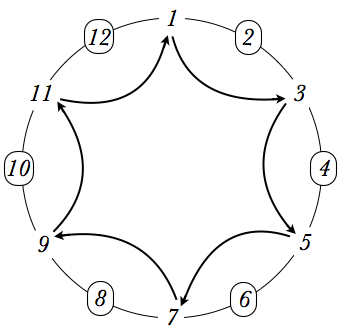
\includegraphics[scale=0.3]{FiguresMaths/josephus12step1}
\caption{The first round of the Josephus erasure process for $n=12$.}
        \label{fig:josephus12step1} 
\end{center}
\end{figure}
The circled numbers in each figure are those that are removed at that round.
\begin{figure}[ht]
\begin{center}
        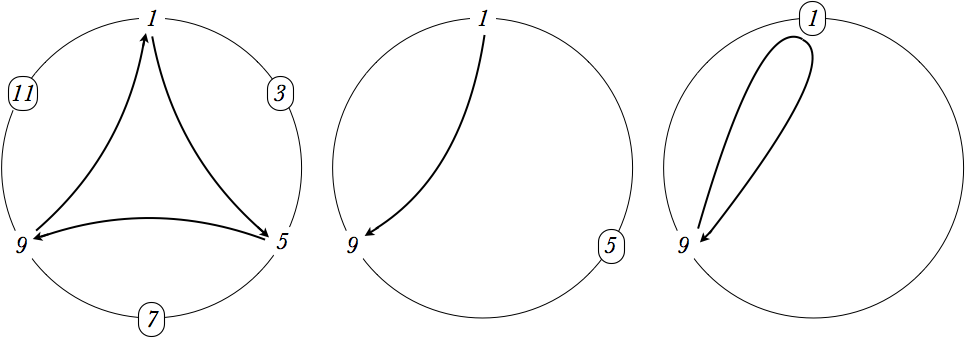
\includegraphics[scale=0.3]{FiguresMaths/josephus12LastSteps}
        \caption{The final rounds of the Josephus erasure process when $n=12$: \ $J(12) = 9$}
        \label{fig:josephus12step2}
\end{center}
\end{figure}
Note that the first round of the process takes $\lceil n/2 \rceil$ steps, while each subsequent round takes ``half" the number of its preceding round---``half" appears in quotes to emphasize the required up-rounding at each halving.

\medskip

{\bf To do}. {\em Prove the following quadripartite proposition which characterizes $J(n)$ for some particular values of $n$.}

\hspace*{.25in}
\begin{tabular}{clll}
 & \underline{Condition on $n$} & \hspace*{.1in} & \underline{Value of $J(n)$} \\ 
{\bf (a)} &
For all $n$ &  & $J(n)$ is odd. \\
{\bf (b)} &
$n$ is even; i.e., $n = 2m$ & & $J(2m) = 2J(m)-1$ \\
{\bf (c)} &
$n$ is odd; i.e., $n = 2m+1$ & & $J(2m+1) = 2J(m)+1$ \\
{\bf (d)} &
$n = 2^m+k$, with $k < 2^m$ & & $J(2^m+k) = 2k+1$
\end{tabular}

The proof proceeds as follows.
\begin{itemize}
\item {\bf (a)} 
All the even numbers are erased in the first round, so only odd numbers remain thereafter.

\medskip
\item {\bf (b)} 
This is a simple generalization of {\bf (a)}.  If $n$ is even, then the first round leads to a circle containing half as many numbers. 
%In other words, rank $i$ becomes rank $(2i-1)$.

\medskip
\item {\bf (c)} 
This is the counterpart of {\bf (b)} for the odd numbers.

\medskip
\item {\bf (d)} 
Observing the successive values for small values of $n$ exposes the relevant pattern.
The values $J(n)$ are grouped by successive powers of $2^m$.  The rule within each group is to start at $1$ and then proceed by increments of $2$ until you reach the next group
($0 \leq k < 2^m$).

\medskip

The formal proof that $J(2^m+k) = 2k+1$ is by induction on $n$.

\smallskip

{\sf Base}.
If $n=1$, then $m=0$, $k=0$ and $J(1) = 2^0+0 = 1$.

\smallskip
 
{\sf Inductive hypothesis}.
Suppose the formula holds for integers $n < 2^m+k$.
\smallskip

{\sf Inductive extension}.
We branch on $k$'s parity:
\begin{itemize}
\item If $k$ is even, then so also is $2^m+k$; therefore, we can write:
\[ J(2^m+k) \ = \ 2J(2^{m-1}+(k/2))-1 \]
By the induction hypothesis, $J(2^{m-1} + (k/2)) = 2(k/2) +1 = k+1$.

Thus, $J(2^m+k) = 2(k+1) -1 = 2k+1$.

\item 
If $k$ is odd, the proof is similar:
\[ J(2^m+k) \ = \ 2J(2^{m-1}+\lfloor k/2 \rfloor)+1 \ = \ 2\lfloor k/2 \rfloor +1 \ = \ 2k+1 \]
\end{itemize}

\end{itemize}

\medskip

{\bf To do}. {\em Provide a closed-form expression for $J(n)$ in terms of $n$'s base-$2$ numeral.}

\medskip

Consider the binary numerals for $n = 2^m +k$ and $k$.  We first note that, {\em numerically},
\begin{eqnarray*}
n & = & 2^m b_m \ + \ 2^{m-1} b_{m-1} \ + \cdots + \ 2 b_1 \ + \ b_0 \\
k & = & 2^{m-1}  b_{m-1} \ + \cdots + \ 2 b_1 \ + \ b_0
\end{eqnarray*} 
where each bit $b_i \in \{0,1\}$.  Therefore, in terms of {\em base-$2$ numerals}:
\[ \begin{array}{ccrl}
(n)_2 & = & 1 b_{m-1} \cdots b_1 b_0 & (\mbox{by definition, } \ b_m=1) \\ 
(k)_2 & = & 0 b_{m-1} \cdots b_1 b_0 & (\mbox{because } [n = 2^m +k] \mbox{ and } k < 2^m)
\end{array}
\]
Therefore:
\[ (J(n))_2 \ = \ b_{m-1} \cdots b_0 b_m. \]

This means that the value of $J(n)$ is obtained by a simple shift to the left of the binary representation of $n$, with a $1$ at the rightmost position.

\smallskip

The pictorial interpretation of this coding is given in Fig.~\ref{fig:josephusCoding} for $n=43$.
\begin{figure}[h]
\begin{center}
        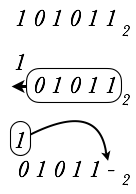
\includegraphics[scale=0.35]{FiguresMaths/josephusCoding}
        \caption{Computing the survivor number $J(43)=23$.}
        \label{fig:josephusCoding}
\end{center}
\end{figure}

\end{itemize}

%%%

\begin{itemize}
\item {\bf 10.5. An alternative to Horner's Rule}

\smallskip

Estrin's method begins with a polynomial of degree $d$ with real coefficients:
\[
P(x) \ \ = \ \ a_0 \ + \ a_1 x \ + \ a_2 x^2 \ + \cdots + \ a_{d-1} x^{d-1} \ + \ a_d x^d
\]
%which is transformed as follows:
%\[
%P(x) \ \ = \ \ a_0 \ + \ x \cdot (a_1 \ + \ x \cdot (a_2  \ +  \cdots                                          
%+ x \cdot (a_{d-2} \ + \ x \cdot (a_{d-1} \ + \ a_d x)) \cdots ))
%\]

We introduce the recursively auxiliary expressions.  
\begin{eqnarray*}
C_i^{(0)} & = & a_i + x a_{i+1} \\
                &\vdots &  \\
C_i^{(n)}  & = & C_i^{(n-1)} + x^{2n} C_{i+2^n}^{(n-1)}
\end{eqnarray*}
The method completes by expressing $P(x)$ in terms of the auxiliary $C_i^{(k)}$
\medskip

{\bf To do}.
\begin{enumerate}
\item
{\em Write $P(x)$ using the auxiliary expressions $C_i$.}  

\smallskip

We simplify expressions by assuming that $d+1$ is a power of $2$
and let develop the method for a degree-$(d=7)$ polynomial.

\begin{eqnarray*}
P_7(x) & = & \ \ a_0 \ + \ a_1 x \ + \ a_2 x^2 \ +  \ a_{3} x^{3} \ + \ a_4 x^4 \ + \ a_{5} x^{5} \ + \ a_{6} x^{6} \ + \ a_7 x^7 \\
& = & \ \ a_0 \ + \ x \cdot a_1 \ + \ x^2 \cdot (a_2  \ + \ x \cdot a_3) \ + \ x^4 \cdot (a_4  \ + \ x \cdot a_5) \ +  \ x^6 \cdot (a_6  \ + \ x \cdot a_7)\\
& = & \ \ (a_0 \ + \ x \cdot a_1) \ + \ x^2 \cdot (a_2  \ + \ x \cdot a_3) \ + \ x^4 \cdot \left( (a_4 \ + \ x \cdot a_5) \ + \ x^2 \cdot (a_6  \ + \ x \cdot a_7) \right) \\
& = & \ C_{0}^{(0)} \ + \ x^2 \ C_2^{(0)} \ + \ x^4 \ ( \ C_4^{(0)} \ + \ x^2 \ C_{6}^{(0)} \ ) \\
& = & C_0^{(1)} \ + \ x^4 \ C_4^{(1)} 
\end{eqnarray*}

The generalization for degree-$d$ polynomials is in the direct line as follows:

\begin{eqnarray*}
P_d(x) & = & \ \ a_0 \ + \ a_1 x \ + \ a_2 x^2 \ +  \ \cdots \ + \ a_{d-1} x^{d-1} \ + \ a_{d} x^{d} \\
& = & \ \ a_0 \ + \ x \cdot a_1 \ + \ x^2 \cdot (a_2  \ + \ x \cdot a_3) \  +  \ \cdots \ + \ x^{d-1} \cdot (a_{d-1}  \ + \ x \cdot a_{d})\\
& = & \ \ (a_0 \ + \ x \cdot a_1) \ + \ x^2 \cdot (a_2  \ + \ x \cdot a_3) \ + \ \cdots \ + \ x^{d-3} \cdot (a_{d-3} \ + \ x \cdot a_{d-2}) \\
& & \ \ + \ x^{d-1} \cdot (a_{d-1}  \ + \ x \cdot a_{d}) \\
& = & \ C_{0}^{(0)} \ + \ x^2 \ C_2^{(0)} \ + \ x^4 \ ( \ C_4^{(0)} \ + \ x^2 \ C_{6}^{(0)} \ )  \ + \ \cdots \\
&  & \ + \ C_{d-7}^{(0)} \ + \ x^2 \ C_{d-5}^{(0)} \ + \ x^4 \ ( \ C_{d-3}^{(0)} \ + \ x^2 \ C_{d-1}^{(0)} ) \\
& = & \ C_{0}^{(1)} \ + \ x^4 \ C_4^{(1)} \ + \ x^8 \ ( \ C_8^{(1)} \ + \ x^4 \ C_{12}^{(1)} \ )  \ + \ \cdots \\
&  &  \ + \ x^{(d+1)-4} \ ( \ C_{(d+1)-4}^{(1)} \ + \ x^4 \ C_{d-1}^{(1)} ) \\
& = & \ C_{0}^{(2)} \ + \ x^8 \ C_8^{(2)}  \ + \ \cdots \ + \ x^{(d+1)-4} \ C_{(d+1)-4}^{(2)} \\
& & \cdots \\
& = & \ C_0^{(log (d-1))} \ + \ x^{{d+1} \over {2}} \ C_{{d+1} \over {2}}^{(log (d-1))} 
\end{eqnarray*}

\medskip
\item
{\em Determine how many additions and multiplications are required to evaluate $P(x)$.}

As before, we focus again on the case on $d=7$ for a detailed analysis. 
\[
P_7(x) \ \ = \ \ C_{0}^{(0)} \ + \ x^2 \ C_2^{(0)} \ + 
\ x^4 \ ( \ C_4^{(0)} \ + \ x^2 \ C_6^{(0)} \ )
\ = \ C_0^{(1)} \ + \ x^4 \ C_4^{(1)} 
\]
We use $2$ multiplications to compute $x^2$ and $x^4$, namely,
$[x^2 \ = \ x \times x]$ and $[x^4 \ = \ x^2 \times x^2]$.

\smallskip

Then, we use $4$ multiplications by $x$ for the four products $a_7 \cdot x$,  $a_5 \cdot x$, $a_3 \cdot x$, and $a_1 \cdot x$.  These are followed by $4$ additions.

\smallskip

Next, we use $2$ multiplications by $x^2$ for the products $x^2 \cdot C_2^{(0)}$ and $x^2 \cdot C_6^{(0)}$.  These are followed by $2$ additions.

\smallskip

Finally, we use $1$ multiplication to compute $x^4 \cdot C_4^{(1)}$.  This is followed by $1$ addition.

\medskip

We have, thus, used a total of $9$ multiplications and $7$ additions.

\medskip

Generalization: 
$\Theta(d + log_2(d))$ multiplications and $\Theta(d)$ additions.
\end{enumerate}

{\Arny We need some guidance for the generalization}
\end{itemize}


%%%%%%%%%%%%%%%%%%%%%%%%%%%%%%%%%%%%%%%%%
% \section{Chapter 11}
\begin{itemize}
\item
{\bf 11.2. Counting replicated triangles}
\smallskip

{\bf To do}.  {\em Determine how the progression of numbers of triangles contained within successive rank-$k$ triangles $T_k$ grows}

\smallskip

Let $N_k$ denote the number of triangles that reside within a rank-$k$ triangle $T_k$.

We have already observed that $N_0 =1$, $N_1 = 5$, and $N_2 = 13$.
  \begin{enumerate}
  \item
{\em Compute} $N_4$.

\smallskip

We begin with a single rank-$4$ triangle $T_4$.

\smallskip

We next observe Fig.~\ref{fig:countingTriangles3}, wherein there are $3$ (partially overlapping) copies of the rank-$3$ triangle $T_3$.
\begin{figure}[h]
\begin{center}
        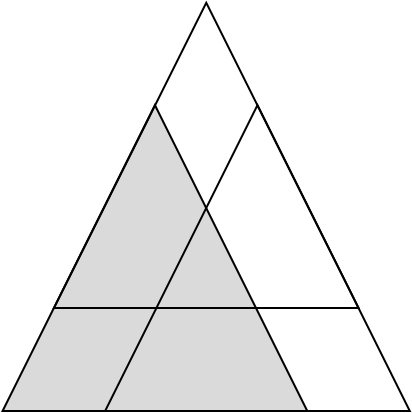
\includegraphics[scale=0.25]{FiguresArithmetic/CountingTriangles3} 
        \caption{The rank-$3$ triangles $T_3$ contained within the rank-$4$ triangle $T_4$.}
        \label{fig:countingTriangles3}
\end{center}
\end{figure}
Next, we inspect Fig.~\ref{fig:countingTriangles2}
\begin{figure}[h]
\begin{center}
        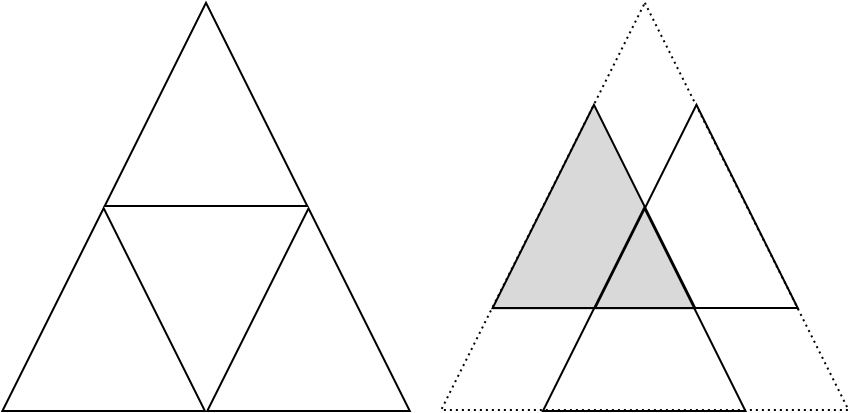
\includegraphics[scale=0.25]{FiguresArithmetic/CountingTriangles2} 
        \caption{$4$ triangles $T_2$(left) and $3$ triangles $T_2$(right).}
        \label{fig:countingTriangles2}
\end{center}
\end{figure}
in order to enumerate the rank-$2$ triangles $T_2$ within $T_3$.  Finally, we focus on the smallest triangle, $T_1$.  Counting them row by row indicates that their number equals the sum of the first $k$ integers (here $k=4$).
This sum is well-known and it is equal to the square of the rank: $4^2 = 16$.

\smallskip

Summing up all levels, we obtain:  $N_4 \ = \ 1 + 3 + 7 + 16 \ = \ 27$.

\medskip\item
{\em Develop a recurrence for} $N_k$ (i.e., the general case).

\smallskip

The recurrence is obtained by generalizing the analysis of the case $k=4$.

\smallskip

For each triangle $T_k$, we have $3$ intertwined triangles $T_{k-1}$ (which contributes, $3 N_{k-1}$ to our count).  Two of these triangles share a common part, which is a copy of triangle $T_{k-2}$; this count (which amounts to $ -3 N_{k-2}$) must be removed from our count, so that we avoid double-counting.  But, there is another part which is common to these three triangles. This part has lower rank and is a copy of $T_{k-3}$ (accordingly we add $+ N_{k-3}$ to our count).  Finally, we must add the largest triangle, $T_{k}$ (which augments our sum by $+1$).  Finally, when $k$ is even,  there is an extra copy of triangle $T_{k-2}$ which appears reversed in the middle of $T_k$ (augments our sum by $+1$ in this case).

\smallskip

In summary, our tally is as follows:\footnote{We added the artificial case $k=0$ in order to simplify the expression}.
\[ N_k \ = \ \left\{
\begin{array}{cl}
3 (N_{k-1} - N_{k-2}) + N_{k-3} + 2 & \mbox{ when $k$ is even} \\
3 (N_{k-1} - N_{k-2}) + N_{k-3} + 1 & \mbox{ when $k$ is odd} \\
5 & \mbox{ when $k=2$} \\
1 & \mbox{ when $k=1$} \\
0 & \mbox{ when $k=0$}
\end{array}
\right. \] 

%For even $k$:  $N_k = 3 (N_{k-1} - N_{k-2}) + N_{k-3} + 1 + 1$
%For odd $k$: $N_k = 3 (N_{k-1} - N_{k-2}) + N_{k-3} + 1$
%with $k \geq 3$ et $N_0 = 0$, $N_1 = 1$ et $N_2 = 5$

\medskip

Courageous readers can verify that this recurrence leads to the following explicit expression for $N_k$:
\[ N_k \ = \ \left\{
\begin{array}{cl}
{1 \over 8} k(k+2)(2k+1) & \mbox{ when $k$ is even} \\ 
{1 \over 8} k(k+2)(2k+1)-{1 \over 8}  & \mbox{ when $k$ is odd}
\end{array}
\right. \]
\end{enumerate}

%%%


\medskip\item
{\bf 11.6. Monge shuffles: mathematical party tricks}

\smallskip

We have introduced two versions of the Monge shuffle.
For both shuffle-techniques. we begin with a deck of $2n$ distinct cards.  
We employ the running example of the following small deck, where $n=4$:
\[ (1, \ 2, \ 3, \ 4, \ 5, \ 6, \ 7, \ 8) \]
For both {\it Monge shuffles} of the cards, we cut the deck in the middle, to create two $n$-card decks:
\[ (1, \ 2, \ 3, \ 4), \ (5, \ 6, \ 7, \ 8) \]
We then merge the two $n$-card decks to again obtain a single $2n$-card deck.  The two Monge shuffles differ in their merging techniques.

  \begin{enumerate}
  \item 
  {\bf The simple Monge shuffle}

\smallskip

The first, simple, Monge shuffle alternates the ``top" cards from the righthand and lefthand $n$-card decks. 
The merged deck has the form
\[ (5, \ 1, \ 6, \ 2, \ 7, \ 3, \ 8, \ 4) \]

{\em Prove the following Proposition.}

{\em Let $p$ be a prime ($p>2$), and let $n = {1 \over 2} (p-1)$.  
Let us begin with a deck of $2n$ distinct cards and perform the simple Monge shuffle on the deck.  
After some number $m$ of cut-then-merge steps, where $m$ divides $p-1$, the simple Monge shuffle replicates the initial deck.}
\smallskip

Let us determine what happens to the card at rank $k$:

The first $n$ cards are simply shifted to ranks $2k$, the $n$ others are moved to ranks $1$, $3$, ... $2n-1$,
thus, $k$ becomes $2k$ modulo $(2n+1)$. 
Similarly, after $i$ such rounds, the k-th card comes at position $2^i$ $[2n+1]$. 

If $2n+1$ is prime, which is the case for a deck of $52$ cards, 
we use the Fermat little theorem to show that the number of rounds required for coming back to the initial position 
divides $p-1$.
Thus, it is equal to $2n$. 

\medskip
\item {\bf The sophisticated Monge shuffle}
\smallskip

We now provide a more sophisticated merge procedure, which yields a sophisticated variant of the Monge shuffle. 
In each stage of this variant---each corresponding to a cut-then-merge step of the simple shuffle---we rearrange the $2n$-card deck directly, from the middle outward, via the following regimen:
\smallskip

\noindent
- Card \#1 of the original deck is placed in position $n+1$ of the shuffled deck \\
- Card \#2 of the original deck is placed in position $n$ of the shuffled deck \\
- Card \#3 of the original deck is placed in position $n+2$ of the shuffled deck \\
- Card \#4 of the original deck is placed in position $n-1$ of the shuffled deck \\
\hspace*{.1in} \ldots and so on, until the original deck is empty.

\smallskip
\ignore{********************************
The first few steps of a stage of the sophisticated Monge shuffle are illustrated for the case $n=4$ in Fig.~\ref{fig:suffleMonge1};
\begin{figure}[h]
\begin{center}
        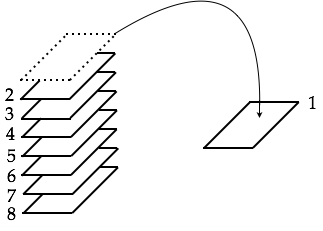
\includegraphics[scale=0.33]{FiguresArithmetic/suffleMongeStep1}
        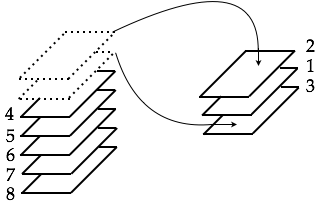
\includegraphics[scale=0.33]{FiguresArithmetic/suffleMongeStep2}
         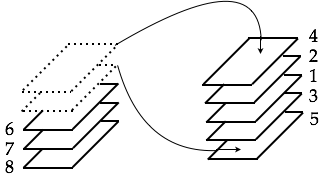
\includegraphics[scale=0.33]{FiguresArithmetic/suffleMongeStep3}
        \caption{The Monge shuffle for $8$ cards ($n=4$): Step 1 (left), Step 2 (center), Step 3 (right).}
        \label{fig:suffleMonge1}
\end{center}
\end{figure}
one complete stage is illustrated in the table following the figure.
\[ \begin{array}{cccccccccccccccccc}
\mbox{Step } & \multicolumn{8}{c}{\mbox{Original deck}} & &
     \multicolumn{8}{c}{\mbox{Shuffled deck}} \\
\hline
1 & (1 & 2 & 3 & 4 & 5 & 6 & 7 & 8) & \rightarrow & ( - & - & - & - & 1 & - &  - & - ) \\
2 & ( - & 2 & 3 & 4 & 5 & 6 & 7 & 8) & \rightarrow & ( - & - & - & 2 & 1 & - & - & - ) \\
3 & ( - & - & 3 & 4 & 5 & 6 & 7 & 8) &  \rightarrow& ( - & - & - & 2 & 1 & 3 & - & - ) \\
4 & ( - & - & - & 4 & 5 & 6 & 7 & 8) &  \rightarrow& ( - & - & 4 & 2 & 1 & 3 & - & - ) \\
5 & ( - & - & - & - & 5 & 6 & 7 & 8) &  \rightarrow& ( - & - & 4 & 2 & 1 & 3 & 5 & - ) \\
6 & ( - & - & - & - & - & 6 & 7 & 8) &  \rightarrow& ( - & 6 & 4 & 2 & 1 & 3 & 5 & - ) \\
7 & ( - & - & - & - & - & - & 7 & 8) &  \rightarrow& ( - & 6 & 4 & 2 & 1 & 3 & 5 & 7 ) \\
8 & ( - & - & - & - & - & - & - & 8) &  \rightarrow& ( 8 & 6 & 4 & 2 & 1 & 3 & 5 & 7 ) \\
\end{array}
\]
*********************************}

{\em Prove the following Proposition.}

{\em For any integer $n \in \N^+$: 
If $4n+1$ is prime, then performing $2n$ steps of the sophisticated Monge shuffle on a deck of $2n$ distinct cards 
restores the deck to its original order.}
\smallskip

Card $1$ goes at position $n+1$, card $2$ goes at $n$, $3$ at $n+1$, ... and card $2n$ goes to position $1$.

This result can be obtained by using again Fermat little theorem.
The place originally occupied by card at rank $k$ is the one whose rank is congruent to $+/- 2k$ modulo $(4n+1)$.
If $4n+1$ is a prime, then, this number divides $2n$.
Thus, $2n$ rounds are needed to restore the original deck. 
\end{enumerate}
  
\end{itemize}


%%%%%%%%%%%%%%%%%%%%%%%%%%%%%%%%%%%

%\section*{Exercises: Chapter 12}


\begin{itemize}
\item
{\bf 12.1. Vertex-degrees and the existence of paths}
\smallskip

{\em Prove that if every vertex of graph $\g$ has degree $\geq d$, then $\g$ contains a {\em simple} path of length $d$.}
\smallskip

Let us consider a \textit{maximal} path in $\g$ (that is a path of maximum length). 

Take an extremity of this path, we denote by $x$ this vertex.
As the path is maximal, all the vertices adjacent to $x$ belong to this path (otherwise, the path will be increased
and it contradicts the maximality).

Every vertices, including $x$, have a degree more than $d$, thus, the path has at least $d$ other vertices.

\medskip\item
{\bf 12.2. Vertex-degrees and their distributions in graphs}
\smallskip

{\em Prove the following result.}

Let $\g$ be an arbitrary graph.
\smallskip

{\bf (b)}
The number of $\g$'s vertices having odd vertex-degree is even.

The solution is obtained by decomposing the sum of the degrees over the odd and even integers.
\[
\sum_{v \in {\cal N}}  =  \sum_{\cal N} odd + \sum_{\cal N} even
\]
\smallskip

We know from proposition~\ref{thm:even-num-odd-degrees} that 
$\sum_{v \in {\cal N}}$ is even and obviously, the sum of even numbers is even,
thus,  the sum of the odd vertices is even.

The only way is that there is an even number of odd vertex-degrees. 

\medskip\item
{\bf 12.8. A small graph isomorphism}
\smallskip

{\em Prove the following Proposition:}
\smallskip

{\em The order-$4$ hypercube $\q_4$ is \textit{isomorphic} to the $4 \times 4$ torus $\widetilde{\m}_{4,4}$.}
\smallskip

%Try to find a relation (an ``encoding") between the bit-strings that name the vertices of $\q_4$ and the ordered pairs of integers that name the vertices of $\widetilde{\m}_{4,4}$.
%\smallskip 
%
%Once you get an idea for how such an ``encoding" might work, try to incorporate the inter-vertex names of edges for both graphs.
%\medskip

$\q_4$ is represented by its natural Gray codes,
where a vertex is coded 4 bits and connected to its four neighbors by complementing 
the digit in each of the four dimensions.
Fig.~\ref{fig:IsomorphismCodingPrinciple}(left) depicts this coding of a vertex and its neighbors.
\medskip

$\widetilde{\m}_{4,4}$ is the cartesian product between two cycles.
Each one is composed of the four vertices connected using the Gray code
$00, 01, 11, 10$.
Fig.~\ref{fig:IsomorphismCodingPrinciple}(right) shows this coding and 
its correspondence with the hypercube. 
The whole coding is obtained by concatenation of both dimensions (horizontal and vertical).
See Fig.~\ref{fig:IsomorphismCodingComplete}
For instance the bottom left vertex is labelled by $00 | 00$. 
\medskip
 \begin{figure}[hbt]
\begin{center}
       \includegraphics[scale=0.45]{FiguresGraph/IsomorphismEx2}
       \caption{Coding schemes for the hypercube and torus.}
  \label{fig:IsomorphismCodingPrinciple}
\end{center}
\end{figure}
 \begin{figure}[hbt]
\begin{center}
       \includegraphics[scale=0.45]{FiguresGraph/IsomorphismEx1}
       \caption{Complete coding schemes.}
  \label{fig:IsomorphismCodingComplete}
\end{center}
\end{figure}

The above description of the codings shows the one-to-one correspondence between the vertices of each graph.
The next step is to show the one-to-one correspondence of the relative edges.


\medskip\item
{\bf 12.9. A traffic map for a mesh-structured city}
\smallskip


  \begin{enumerate}
  \item
In the {\em metro} version of the model, we pay a fee every time we encounter a new site on the way from $\langle i,j \rangle$ to $\langle h,k \rangle$.

\smallskip

{\em What is the cost of a trip from a site $\langle i,j \rangle$ to the most-distant site, $\langle h,k \rangle$, under the metro model?}
\smallskip

We should first characterize which vertex is the most distant from $\langle i,j \rangle$. 
Of course, the answer will depend on where this vertex is located in its quadrant.

Let us restrict (without loss of generality) to any quadrant, say the right-bottom one. 
There are two situations to consider that are illustrated in Fig.~\ref{fig:routingWorstCase}
where the shaded area distinguish the location of the destination $\langle h,k \rangle$.
The first situation (left in the figure) is easy since the directions of the edges allow $\langle i,j \rangle$ to reach directly $\langle h,k \rangle$
without going out of the considered quadrant while in the second situation (right on the figure) we should reach an external
vertex in the bottom-left quadrant, then, reach a vertex in the top-left one, then, reach a vertex in the top-right before being able to
reach $\langle h,k \rangle$.
The worst case comes from this last situation where the internal paths are maximized (see Fig.~\ref{fig:routingCitySolution}).

  \medskip\item
In the {\em driving} version of the model, we pay a per-kilometer fee of $n^{(1/2)^\ell}$ units every time we traverse a level-$\ell$ edge on the way from $\langle i,j \rangle$ to $\langle h,k \rangle$.
 \smallskip


{\em What is the cost of a trip from a site $\langle i,j \rangle$ to the most-distant site, $\langle h,k \rangle$, under the driving model?}
\smallskip

 The previous analysis still holds. 
 \end{enumerate}
  \begin{figure}[hbt]
\begin{center}
       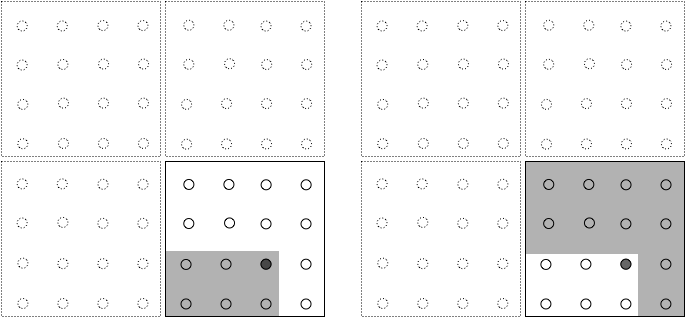
\includegraphics[scale=0.4]{FiguresGraph/routingWorstCase}
       \caption{The two possible situations for reaching a vertex in the same bottom-right quadrant.
       The origin vertex $\langle i,j \rangle$ is represented in dark grey and the destination vertex is on the shaded quadrant.}
  \label{fig:routingWorstCase}
\end{center}
\end{figure}

 \begin{figure}[hbt]
\begin{center}
       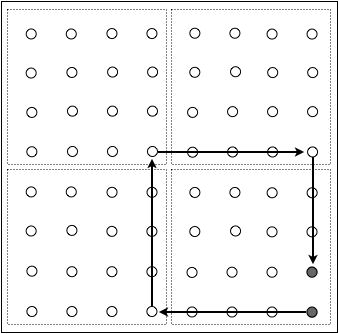
\includegraphics[scale=0.4]{FiguresGraph/routingCitySolution}
       \caption{Worst case in the metro model.}
  \label{fig:routingCitySolution}
\end{center}
\end{figure}

\ignore{************ 
 \begin{figure}[hbt]
\begin{center}
       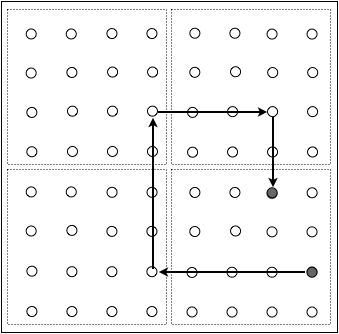
\includegraphics[scale=0.4]{FiguresGraph/routingCitySolution1}
       \caption{To discuss.}
  \label{fig:routingCity}
\end{center}
\end{figure}
 \begin{figure}[hbt]
\begin{center}
       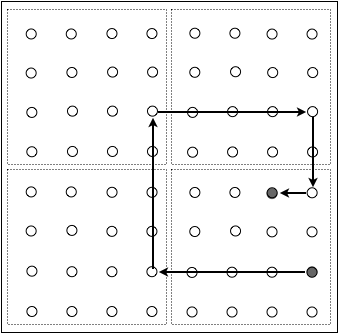
\includegraphics[scale=0.4]{FiguresGraph/routingCity2}
       \caption{To discuss.}
%  \label{fig:routingCity}
\end{center}
\end{figure}
 \begin{figure}[hbt]
\begin{center}
       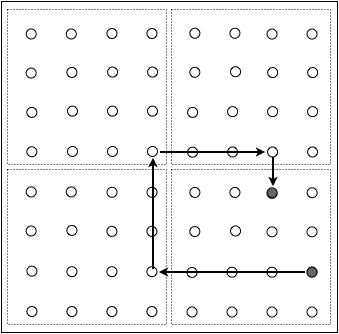
\includegraphics[scale=0.4]{FiguresGraph/routingCity3}
       \caption{Shortest path.}
%  \label{fig:routingCity}
\end{center}
\end{figure}
************}

\end{itemize}


%%%%%%%%%%%%%%%%%%%%%%%%%%%%%%%%%%%%%%%%
%\section*{Exercises Chapter 13}

\begin{itemize}
\item
{\bf 13.2. Appreciating de Bruijn networks}

\smallskip

{\bf To do}.
{\em Identify, by coloring the edges of $\d_3$, how the network can be viewed as two directed trees which are ``embracing" one another.}

\smallskip

Being constrained to ``monochromaticism", we partition $\d_3$ into two isomorphic sub-digraphs, which are the sought ``red" and ``green" directed trees of the problem.  Fig.~\ref{fig:DeBruijn3Tree} depicts both trees.  The tree in the left side of the figure is rooted at its leftmost vertex;  the tree in the right side of the figure is rooted at its rightmost vertex. 
\begin{figure}[h]
\begin{center}
        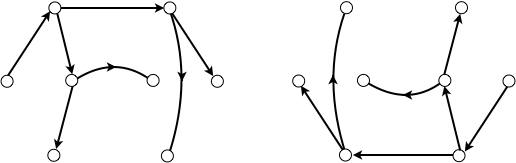
\includegraphics[scale=0.4]{FiguresGraph/DeBruijn3Tree}
        \caption{Two disjoint trees that cover $\d_3$ in an interleaved manner.}
        \label{fig:DeBruijn3Tree}
\end{center}
\end{figure}

\smallskip

Hopefully, the reader has a feeling of how this covering can be extended beyond order $3$.  Actually depicting the relevant trees is a daunting task, because drawing any network $\d_k$ for $k > 3$ is a daunting task.

\medskip\item 
{\bf 13.4. Fundamental insights into outerplanarity in graphs}
\smallskip

{\em Prove the following assertions.}

\noindent {\em a. Show that the complete bipartite graph $K_{3,2}$ is not outerplanar.}

\smallskip

The question is how to distribute the two groups of vertices (dark grey and white) on a circle
with no crossing edges.
The solution is a case by case analysis according to all the possibilities to distribute $K_{3,2}$'s vertices around a circle:
either the vertices of each of both groups are distributed consecutively, or each group of vertices is interlaced with a vertex of the other group.
Fig.~\ref{fig:outerplanarK32} depictes both cases.

It is easy to verify that in each case, it is impossible to link the isolated white vertex with all the three dark grey ones.

\begin{figure}[h]
\begin{center}
        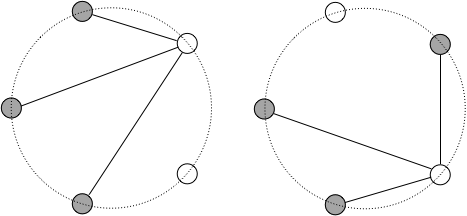
\includegraphics[scale=0.4]{FiguresGraph/outerplanarK3,2}
        \caption{The two only possibilities to distribute the white and shaded vertices along a circle.}
        \label{fig:outerplanarK32}
\end{center}
\end{figure}


\end{itemize}


